% !TeX root = ../main.tex
% Add the above to each chapter to make compiling the PDF easier in some editors.

\chapter{Methodik}\label{chapter:Methodik}
In diesem Kapitel werden Hypothesen aufgestellt, die später anhand des vorliegenden Datensatzes ausgewertet und überprüft werden. Sie ermöglichen es, die Daten in bestimmten Bereichen detaillierter zu betrachten. Des weiteren wird die Bewertungsmethodik vorgestellt, die angewendet wird, um die aufgetretenen Unfälle bezüglich ihres Risikos zu bewerten. Die bewerteten Unfälle werden anschließend auf beispielhafte Fahrsituationen im Untersuchungsgebiet übertragen.

\section{Hypothesen}\label{section:Hypothesen}
Anhand der vorausgegangenen Literaturrecherche kann eine Vielzahl an Hypothesen bezüglich Situationen und Eigenschaften, die ein höheres Unfallrisiko mit sich bringen, aufgestellt werden. Im Rahmen dieser Arbeit werden Hypothesen aufgestellt, die später mit den vorliegenden Unfalldaten verglichen und auf ihre Gültigkeit überprüft werden. Im Fokus vieler Unfallforschungen steht vielmals das Alter oder die Aufmerksamkeit der Unfallbeteiligten, auch spielt die Geschwindigkeitsüberschreitung häufig eine wichtige Rolle. Diese Punkte werden hier nicht weiter beachtet, da sie bei den vorhandenen Unfalldaten nicht gegeben sind. Des weiteren wird der Einfluss von berauschenden Mitteln nicht weiter analysiert. Dieser Punkt wird vernachlässigt, da später kritische Situationen mit einem menschlichen Fahrer, mit automatisierten Fahrsituationen verglichen werden sollen. Der Zustand des Fahrers ist beim vollautomatisierten Fahren nicht von Bedeutung und wird im Folgenden nicht weiter berücksichtigt. Um Unfälle kritischen Fahrsituationen zuordnen zu können muss man die Unfälle detailliert betrachten. Der Unfalltyp allein reicht dafür nicht aus. Deshalb sind auch die Hypothesen zum Teil sehr spezifisch und orientieren sich größtenteils an den von der Polizei angegebenen Unfallursachen.

Das innerstädtische Straßennetz wird von Knotenpunkten geprägt, an denen viele verschiedene Fahrsituationen auftreten. Bei Abbiegevorgängen handelt es sich dabei um Situationen, die viele Konfliktpunkte aufweisen. Die Zahlen des Statistischen Bundesamtes in \ref{chapter:Unfallursachen innerorts} deuten an, dass es Unterschiede zwischen den Unfallhäufigkeiten beim Links- und Rechtsabbiegen gibt.

\begin{itemize}
	\item Bei der Fahrsituation Linksabbiegen treten im Vergleich zur Situation Abbiegen nach rechts mehr Konfliktpunkte auf. Daher kommt es beim Linksabbiegen häufiger zu Unfällen. (\textit{Hypothese 1})
\end{itemize}

Kapitel \ref{chapter:Knotenpunkte mit LSA} geht auf Konfliktpunkte an Knotenpunkten mit LSA ein. Zudem werden Möglichkeiten diskutiert, wie diese, anhand von Anpassungen der Signalsteuerung, reduziert werden können. Es wird angenommen, dass:
	
\begin{itemize}	
	\item die Konfliktpunkte und Unfallzahlen reduziert werden können, wenn Linksabbieger an Kreuzungen mit \ac{LSA} auf einem eigenen Fahrstreifen mit eigener Signalphase geführt werden. (\textit{Hypothese 2})
\end{itemize}

Es kommt im urbanen Raum jedoch nicht nur zu Unfällen durch Abbiegemanöver. Vor allem bei dichtem Verkehr dürfen Unfälle im Längsverkehr nicht vernachlässigt werden. In Kapitel \ref{chapter:Knotenpunkte mit LSA} wurden solche Unfälle bereits erläutert. Dies führt zur Annahme, dass:

\begin{itemize}	
	\item bei höherem Verkehrsaufkommen, z.B. in den Hauptverkehrszeiten, die Anzahl der Verkehrsunfälle im Längsverkehr steigt. Ursachen dafür sind Konflikte beim Spurwechsel und zu geringer Sicherheitsabstand. (\textit{Hypothese 3})
\end{itemize}	

Bis jetzt wurden nur Hypothesen aufgestellt, die sich mit dem fließenden Verkehr befassen. Im urbanen Raum kommt es zudem häufig zu Unfällen mit Fahrzeugen im ruhenden Verkehr. Kapitel \ref{Urabane Fahrsituationen mit geringen Geschwindigkeiten} befasst sich mit Bereichen, in denen sich Konflikte beim Ein-/Ausparken ereignen. Diese Konfliktpunkte werden in der folgenden Hypothese berücksichtigt.

\begin{itemize}	
	\item Im urbanen Raum kommt es häufig zu Konflikten mit Fahrzeugen im ruhenden Verkehr. Besonders auffällig sind Bereiche mit Längsaufstellung am Fahrbahnrand. Zusätzlich spielt verbotswidriges auf der Straße Halten/Parken, z.B. Parken in zweiter Reihe, eine bedeutende Rolle. Beim Vorbeifahren entstehen kritische Situationen, die zu Unfällen führen. (\textit{Hypothese 4})
\end{itemize}

Urbane Fahrsituationen werden zusätzlich von nicht motorisierten Verkehrsteilnehmern beeinflusst. In Kapitel \ref{subsection:Verkehrsbeteiligung an Unfällen im urbanen Raum} wurde die Verletzungsschwere nicht motorisierter Verkehrsteilnehmer diskutiert. Motorräder und Mopeds weisen oft ähnlich schwere Verletzungen wie Fußgänger und Radfahrer auf und werden in dieser Arbeit zu den nicht motorisierten Verkehrsteilnehmern gezählt. Hierbei muss berücksichtigt werden, dass:
	
\begin{itemize}
	\item die Komplexität einer Fahrsituation und somit auch die Zahl der Unfälle erhöht wird, wenn nicht motorisierte Verkehrsteilnehmer daran beteiligt sind. Durch den geringen Schutz von nicht motorisierten Verkehrsteilnehmern ist der Verletzungsgrad höher als bei Unfällen, an denen nur motorisierte Verkehrsteilnehmer beteiligt sind. (\textit{Hypothese 5})
\end{itemize}

In Kapitel \ref{subsection:Konfliktpunkte zwischen Kraftfahrzeugen und Radfahrern} wurden Abbiegevorgänge vorgestellt, die häufig zu Konflikten mit ungeschützten Verkehrsteilnehmern führen. Hierbei muss berücksichtigt werden, dass:

\begin{itemize}
	\item wenn sich Fußgänger und Radfahrer parallel zum Fahrzeug bewegen es beim Rechtsabbiegen häufiger zu Unfällen kommt als beim Linksabbiegen. Kritische Situationen treten vor allem dann auf, wenn Radfahrer den Radweg in die falsche Richtung befahren. (\textit{Hypothese 6})
\end{itemize}	

Betrachtet man nur die Unfälle, an denen Radfahrer beteiligt sind, gibt es, laut Kapitel \ref{subsection:Charakteristiken und Besonderheiten von Unfällen im urbanen Raum}, Unterschiede, auf was für einer Art von Radverkehrsanlage sich die Radfahrer bewegen.
	
\begin{itemize}	
	\item Bei baulich von der Fahrbahn getrennten Radverkehrsanlagen kommt es häufiger zu Unfällen als bei Radverkehrsanlagen auf der Fahrbahn. Die Unfallgefahr wird durch schlechte bzw. nicht vorhandene Markierungen der Radverkehrsanlagen, besonders im Bereich von Knotenpunkten, erhöht. (\textit{Hypothese 7})
\end{itemize}	
	
In Kapitel \ref{chapter:Unfallursachen innerorts} wurde das fehlerhafte Verhalten der Fußgänger analysiert. Daraus ergibt sich, dass:
	
\begin{itemize}	
	\item falsches Verhalten der Fußgänger häufig die Ursache für Unfälle mit Personenschaden im urbanen Raum ist. Besonders häufig treten die Ursachen Rotlichtverstöße und Überschreiten der Fahrbahn ohne auf den Fzg.-Verkehr zu achten auf. Häufig ereignen sich solche Unfälle in der Nähe von Haltestellen des ÖPNVs. (\textit{Hypothese 8})
\end{itemize}	

Neben den Unfallursachen, die Fahrzeugführern oder Fußgängern zugeschrieben werden können, gibt es auch allgemeine Ursachen, die von den Straßenverhältnissen, Witterungseinflüssen oder Hindernissen im Straßenraum beeinflusst werden. Hier kommt es vor allem: 

\begin{itemize}	
	\item bei Sichtbehinderungen durch Witterungseinflüsse bei der Unfallursache \enquote{Blendende Sonne} vermehrt zu Unfällen. (\textit{Hypothese 9})
\end{itemize}

Die hier aufgeführten Hypothesen werden in Kapitel \ref{sechtion:Überprüfung der Thesen} anhand der Unfalldaten des Testgebiets ausgewertet und überprüft. Hier soll jedoch schon darauf hingewiesen werden, dass die Ergebnisse aufgrund der eher geringen Unfallzahlen im Testgebiet und teilweise unvollständigen Daten nicht vollständig auf andere Bereiche übertragbar sind.


\section{Vorgehen zur Bewertung urbaner Fahrsituationen}\label{section:Bewertung urbaner Fahrsituationen}
Unfälle im urbanen Raum sind zahlreich und ihnen liegen viele verschiedene Fahrsituationen zugrunde. Hierbei gibt es Situationen, die ein erhöhtes Risiko aufweisen, wenn sich ein Unfall ereignet und auch Situationen, denen eher ein geringes Risiko zugeordnet wird. Eine Bewertungsskala ist hilfreich, Unfälle bzw. Fahrsituationen bezüglich ihrer Sicherheitsrelevanz zu klassifizieren. Deshalb wird in diesem Kapitel, basierend auf den Ergebnissen aus Kapitel \ref{section:Ansätze zur Bewertung von Fahrsituationen}, eine Methode zur Bewertung von urbanen Fahrsituationen entwickelt.

\subsection{Vorgehen zur Typisierung von Unfällen}\label{subsection:Vorgehen zur Typisierung}
Der vorhandene Datensatz enthält unterschiedlich ausführliche Angaben. Zu Unfällen, bei denen sich ein Personenschaden oder ein schwerwiegender Sachschaden im engeren Sinne ereignete, liegen ausführlichere Informationen vor, als zu denjenigen, die nicht in diese beiden Kategorien passen. Liegen weniger ausführliche Angaben vor, handelt es sich um eine Kurzaufnahme eines Unfalls. Diese Unfälle werden im folgenden als Kleinunfall bezeichnet. Bei einer Kurzaufnahme werden lediglich Datum, Uhrzeit, Ort und allgemeine Ursachen des Unfalls im Aufnahmeformular angegeben. Anhand dieser Informationen lässt sich der Unfallhergang jedoch nur schwer nachvollziehen. Hierfür eignen sich Beschreibungen des Unfalls, welche nachträglich bei der Polizei München angefragt wurden. Aus Datenschutzgründen konnten jedoch nur Beschreibungen (Kurzsachverhalte) für die Jahre 2013 bis 2016 zur Verfügung gestellt werden. Daher wird bei der Typisierung der Unfälle und der folgenden Bewertung in Kapitel \ref{section:Zuordnung der Unfälle zu Fahrsituationen} nur ein Datensatz über vier Jahre berücksichtigt.

Die Unfälle, die sich im Testgebiet ereigneten, sollen typisiert werden, um die Häufigkeit eines bestimmten Unfalltyps zu bestimmen. Hierfür kann man zunächst die sieben Unfalltypen verwenden. Diese sind jedoch sehr allgemein gehalten. Es wird z.B. nur angegeben, dass es sich um einen Abbiege-Unfall handelt. Unklar ist, ob dieser sich beim Abbiegen nach rechts oder nach links ereignet hat und wer an dem Unfall beteiligt war. Deshalb werden hier die Unfalltypen nach GDV herangezogen, sie wurden z.T. bereits in Kapitel \ref{section:urbane Fahrsituationen und ihre Sicherheitsbewertung} vorgestellt. Alle Feintypen sind in den Abbildungen \ref{fig:FT1} bis \ref{fig:FT7} in Anhang \ref{chapter:Anhang1} dargestellt.

In dieser Arbeit wird zunächst den Unfällen ein Feintyp zugeordnet, bei denen bereits ein Unfalltyp angegeben wurde (keine Kleinunfälle). Hierfür werden die Kurzsachverhalte einzeln durchgearbeitet und mit den Angaben im Unfallprotokoll verglichen. Bei sich widersprechenden Angaben werden die Angaben der Kurzsachverhalte herangezogen. Wurde bei einem Unfall z.B. der Unfalltyp Abbiege-Unfall angegeben, in dem Kurzsachverhalt wurde jedoch ein Unfall beschrieben, bei dem es zu einem Zusammenstoß mit einem von links kommenden Fahrzeug und einem Rechtsabbieger kommt, wird dem Unfall der Feintyp 303 (siehe Abbildung \ref{fig:Einbiege-Unfall}) zugeordnet.

Anschließend werden die Kleinunfälle betrachtet. Hier sind in erster Linie die Kurzsachverhalte für die Zuordnung der Feintypen relevant. Sie werden zusätzlich mit der angegebenen allgemeinen Ursache und dem Unfallort abgeglichen. Hierfür werden die Kurzsachverhalte wieder einzeln durchgearbeitet. Bei einem Unfall wurde z.B. folgendes angegeben: \enquote{Zum Unfallzeitpunkt befuhr die 02 die Rheinstraße in östlicher Richtung. An der Kreuzung Rheinstraße/Leopoldstraße wollte die 02 nach links in die Leopoldstraße abbiegen. Dazu ordnete sie sich auf der Linksabbiegerspur ein. Auch die 01 hatte dieselbe Absicht und befuhr hinter der 02 die Linksabbiegerspur. Bei grünem Licht der LZA fuhr die 02 in den Kreuzungsbereich ein, musste verkehrsbedingt bremsen. 01 konnte ihren Wagen nicht mehr zum Stillstand bringen und fuhr mangels Sicherheitsabstandes auf den Pkw der 02 auf.} Hierbei handelt es sich um einen Unfall dem der Feintyp 201 in Abbildung \ref{fig:Abbiege-Unfall} zugeordnet wird.

Teilweise sind die Beschreibungen sehr kurz gehalten und geben keine detaillierte Auskunft. Es ist daher mit dieser Methode nicht möglich, alle Unfälle mit Feintypen zu typisieren. Die Anzahl der Unfälle, denen kein Feintyp zugeordnet werden kann, ist jedoch gering. Das Lesen der Kurzsachverhalte ist mit großem Aufwand verbunden. Daher ist es für größere Datensätze denkbar, den Feintypen Wortgruppen zuzuordnen, nach denen dann gefiltert wird. %Diese Methode wurde hier nicht angewendet. % Evtl noch mehr dazu schreiben?

\subsection{Bewertungsskala}\label{subsection:Bewertungsskala}
Die Unfälle innerhalb des Testgebiets sollen bezüglich ihrer Sicherheitsrelevanz bewertet werden. Hierfür werden zunächst die Unfälle betrachtet, denen bei der Unfallaufnahme ein Unfalltyp zugeordnet wurde. Im weiteren Verlauf wird die Häufigkeit der typisierten Unfälle berechnet. Durch die Typisierung fließen nun auch die Kleinunfälle mit in die Berechnung ein, die gesamte Anzahl der Unfälle nimmt daher deutlich zu. Zuerst werden nur die sieben Unfalltypen betrachtet, dann wird die Anzahl der Unfälle mit einem bestimmten Feintyp auf die gesamte Anzahl der Unfälle im Testgebiet bezogen. Bei der Gesamtanzahl wird zwischen zwei Fällen unterschieden. Der erste Fall betrachtet nur die Unfälle, die ausführlich aufgenommen wurden. Bei diesen kam es zu einem Personenschaden oder Sachschaden im engeren Sinne, siehe Formel \ref{equation:Häufigkeit(1)}. Der zweite Fall dagegen berücksichtigt alle Unfälle im gesamten Untersuchungsgebiet (Formel \ref{equation:Häufigkeit(2)} und \ref{equation:Häufigkeit(3)}).

\begin{equation}\label{equation:Häufigkeit(1)}
\text{Häufigkeit(x)} = \dfrac{\text{Anzahl Unfälle mit Unfalltyp x}}{\text{Anzahl Unfälle mit P \& S}}*100
\end{equation}

\begin{equation}\label{equation:Häufigkeit(2)}
\text{Häufigkeit(x)} = \dfrac{\text{Anzahl Unfälle mit Unfalltyp x}}{\text{Anzahl Unfälle gesamt}}*100
\end{equation}

\begin{equation}\label{equation:Häufigkeit(3)}
\text{Häufigkeit(x)} = \dfrac{\text{Anzahl Unfälle mit Feintyp x}}{\text{Anzahl Unfälle gesamt}}*100
\end{equation}\\

Die Anzahl der Unfälle für die Jahre 2013 bis 2016 haben im Testgebiet folgende Werte:

\begin{itemize}
	\item Anzahl Unfälle mit P \& S = 591 Stück
	\item Anzahl Unfälle gesamt = 1779 Stück
\end{itemize}

Die so berechnete Häufigkeit der einzelnen Unfalltypen bzw. Feintypen wird nun einem gewissen Bereich der Eintrittswahrscheinlichkeit zugeordnet. Hierfür stehen die vier Bereiche \textit{sehr selten}, \textit{selten}, \textit{oft} und \textit{sehr oft} zur Verfügung. Dieses Vorgehen orientiert sich an dem Risikograph nach DIN V 19250, welcher in Kapitel \ref{subsection:Risikograph} vorgestellt wurde. Um eine sinnvolle Einteilung der  vier Bereiche zu erhalten, erfolgt dies jeweils unter Berücksichtigung der Anzahl der verschiedenen Unfalltypen bzw. Feintypen und der gesamten Anzahl der Unfälle. Tabelle \ref{tab:Haeufigkeits Bereiche} stellt die Eintrittsbereiche dar, die im Verlauf der Arbeit auf die drei oben genannten Fälle angewendet werden.

\begin{table}[htpb]
	\scriptsize
	\caption[Eintrittswahrscheinlichkeit der Unfälle im Testgebiet bei der Betrachtung von Unfalltypen und Feintypen]{Eintrittswahrscheinlichkeit der Unfälle im Testgebiet bei der Betrachtung von Unfalltypen und Feintypen}\label{tab:Haeufigkeits Bereiche}
	\centering
		\begin{tabular}{p{2cm} l l l l}
			\toprule
			Fall & sehr selten & selten & oft & sehr oft \\
			\midrule
			Unfalltypen für S \& P & 0 \% < 7 \%  & 7 \% < 14 \% & 14 \% < 21 \% & 21 \% < 28 \%\\
			Unfalltypen mit K & 0 \% < 11 \%  & 11 \% < 22 \% & 22 \% < 33 \% & 33 \% < 44 \%\\
			Feintypen & 0 \% < 0,5 \% & 0,5 \% < 1,5 \% & 1,5 \% < 3 \% & 3 \% < 8 \%\\
			\bottomrule
		\end{tabular}
\end{table}

Bis jetzt wurden die Unfälle nur anhand der Häufigkeit ihres Auftretens bewertet. Es sind jedoch nicht nur die Unfälle sicherheitsrelevant, welche am häufigsten vorkommen, sondern auch solche, die schwere Folgen haben. Besonders kritisch sind Unfälle, die häufig auftreten und zu schweren Folgen führen. Deshalb wird zusätzlich die Unfallschwere angegeben. Aus den oben genannten Formeln ergeben sich nun die Formeln \ref{equation:Häufigkeit(4)}, \ref{equation:Häufigkeit(5)} und \ref{equation:Häufigkeit(6)}.

\begin{equation}\label{equation:Häufigkeit(4)}
\text{Häufigkeit(xy)} = \dfrac{\text{Anzahl Unfälle mit Unfalltyp x und Unfallschwere y}}{\text{Anzahl Unfälle mit P \& S}}*100
\end{equation}

\begin{equation}\label{equation:Häufigkeit(5)}
\text{Häufigkeit(xy)} = \dfrac{\text{Anzahl Unfälle mit Unfalltyp x und Unfallschwere y}}{\text{Anzahl Unfälle gesamt}}*100
\end{equation}

\begin{equation}\label{equation:Häufigkeit(6)}
\text{Häufigkeit(xy)} = \dfrac{\text{Anzahl Unfälle mit Feintyp x und Unfallschwere y}}{\text{Anzahl Unfälle gesamt}}*100
\end{equation}\\

Bei den vorliegenden Daten wird nicht immer der Wert des entstandenen Sachschadens angegeben. Zudem werden die Verletzungen der Unfallbeteiligten nicht erläutert. Es ist also nicht möglich, die Unfallschwere anhand eines Geldbetrags zu beurteilen. Deshalb wird sie in fünf fixe Kategorien eingeteilt, die die Unfallschwere verdeutlichen. Es wird unterschieden zwischen \ac{K}, \ac{S}, \ac{lvl}, \ac{svl} und \ac{tot}. Die genannte Reihenfolge nimmt in der Schwere zu. Anhand der Unfallschwere und der Häufigkeit ist es jetzt möglich, Unfälle bezüglich ihrer Kritikalität zu bewerten. Hierfür werden in Abbildung \ref{fig:Bewertungsskala} Werte von a bis g zugeordnet. Das mit dem Unfall verbundene Risiko bzw. die Kritikalität steigt von a bis g an. Somit ist es möglich, Unfällen eine bestimmte Risiko-Kategorie zuzuordnen.

\begin{savenotes}
	\begin{figure}[H]
		\centering
		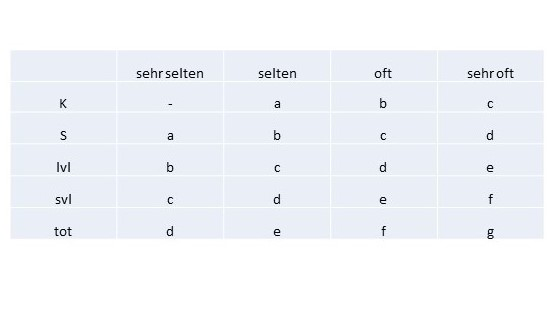
\includegraphics[width=10.6cm,height=3cm]{figures/Bewertungsskala}
		\caption[Bewertungsskala zur Klassifizierung von Unfällen im urbanen Raum]{Bewertungsskala zur Klassifizierung von Unfällen im urbanen Raum}\label{fig:Bewertungsskala}
	\end{figure}
\end{savenotes}

Zur besseren Veranschaulichung können die ermittelten Häufigkeiten, mit Bezug zur jeweiligen Unfallschwere, auch in einem Diagramm dargestellt werden. In Kapitel \ref{subsection:Risikoverteilung auf Unfalltypen} wurde erläutert, wie \Textcite[S. 60]{Gschwendtner.2015} Unfalltypen anhand einer Risikoverteilung bewertet. So eine Risikoverteilung wird auch in dieser Arbeit verwendet. Hierfür wird auf der x-Achse die Häufigkeit eingetragen, die Bereiche werden dabei entsprechend Tabelle \ref{tab:Haeufigkeits Bereiche} angepasst. Auf der y-Achse werden die fünf Unfallschweregrade, der Schwere nach aufsteigend, angegeben. Damit es auch hier möglich ist, die zugehörige Kritikalität abzulesen, werden Risikoäquivalenten eingezeichnet. Den Bereichen zwischen den Risikoäquivalenten werden die gleichen Werte wie in Abbildung \ref{fig:Bewertungsskala} zugeordnet.

\begin{savenotes}
	\begin{figure}[H]
		\centering
		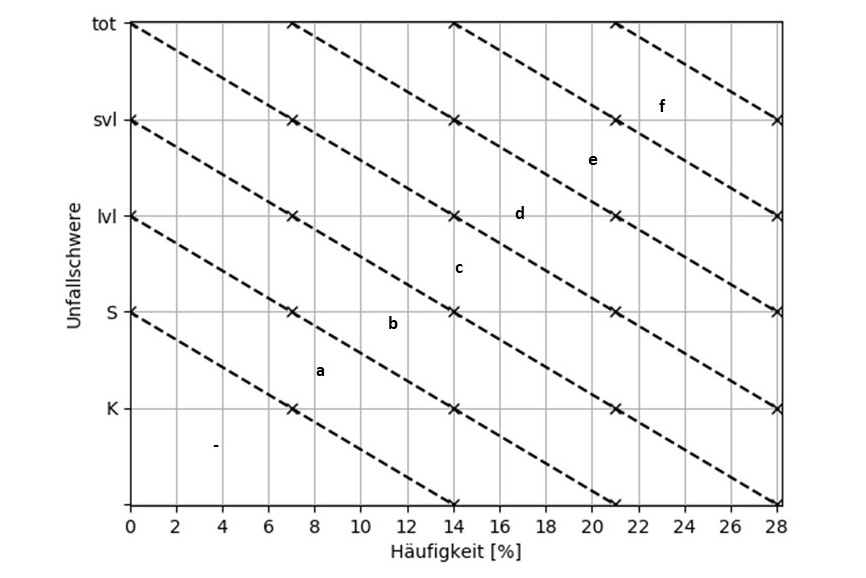
\includegraphics[width=10.5cm,height=7cm]{figures/Bewertungsdiagramm}
		\caption[Bewertungsdiagramm mit Risikoäquivalenten bei gleichmäßiger Verteilung der Häufigkeiten]{Bewertungsdiagramm mit Risikoäquivalenten bei gleichmäßiger Verteilung der Häufigkeiten}\label{fig:Bewertungsdiagramm}
	\end{figure}
\end{savenotes}

Abbildung \ref{fig:Bewertungsdiagramm} stellt ein Diagramm für die Bewertung der Unfalltypen ohne die Berücksichtigung der Kleinunfälle dar, Abbildung \ref{fig:Bewertungsdiagramm(2)} für die der Feintypen. Bei den gestrichelten Linien handelt es sich um die Risikoäquivalenten. Diese wurden anhand der vier Bereiche (sehr selten, selten, oft und sehr oft) in Tabelle \ref{tab:Haeufigkeits Bereiche} ermittelt. Um die Risikoäquivalenten zu erhalten wurde über die Fixpunkte, welche in Tabelle \ref{tab:Haeufigkeits Bereiche} festgelegt wurden, linear interpoliert. Ihnen liegt daher die Funktion $f(x) = \alpha + \beta*x$ zugrunde. Die Fixpunkte wurden in den Abbildungen \ref{fig:Bewertungsdiagramm} und \ref{fig:Bewertungsdiagramm(2)} mit einem x gekennzeichnet. 

\begin{savenotes}
	\begin{figure}[H]
		\centering
		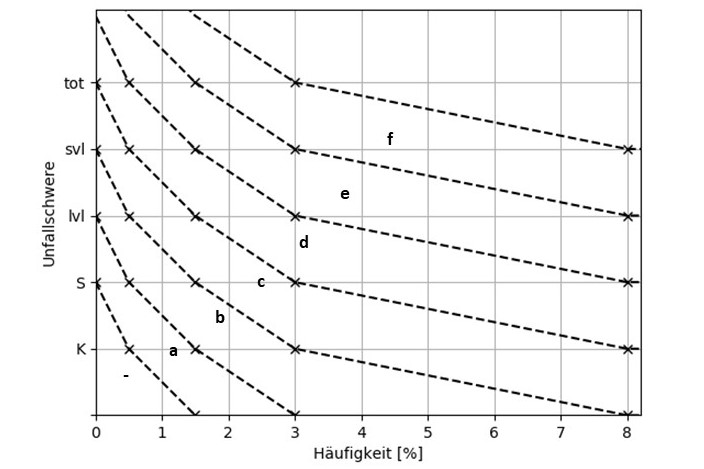
\includegraphics[width=10.5cm,height=7cm]{figures/Bewertungsdiagramm(2)}
		\caption[Bewertungsdiagramm mit Risikoäquivalenten bei ungleichmäßiger Verteilung der Häufigkeiten]{Bewertungsdiagramm mit Risikoäquivalenten bei ungleichmäßiger Verteilung der Häufigkeiten}\label{fig:Bewertungsdiagramm(2)}
	\end{figure}
\end{savenotes}

Ein Unfalltyp bzw. Feintyp kann aufgrund der unterschiedlichen Schweregrade bis zu fünfmal bewertet werden. Sie kommen daher auch in der bildlichen Darstellung in Diagrammen häufiger vor. Maßgebend ist der Eintrag, dem die größte Risiko-Kategorie zugeteilt wird und der somit das höchste Risiko mit sich bringt. Der Unfalltyp 7 kann z.B. einmal mit \textit{b}, aufgrund der Unfälle mit Leichtverletzten, und einmal mit \textit{d}, aufgrund der Unfälle mit Sachschaden, bewertet werden. Maßgeblich ist dann die höhere Risiko-Kategorie \textit{d}.

\subsection{Bewertung urbaner Fahrsituationen}\label{subsection:Bewertungs urbaner Fahrsituationen}
Bis jetzt wurden nur Unfälle bewertet, die sich bereits ereignet haben. Ziel dieser Arbeit stellt jedoch die Bewertung von urbanen Fahrsituationen dar. Anhand der Unfalltypen ist es möglich, Fahrsituationen zu bestimmen, in denen es zu einem Unfall mit einem gewissen Unfalltyp kommen kann. Hierfür werden nur die Unfälle betrachtet, denen ein Feintyp zugeordnet wurde. Die Feintypen werden bereits im Unfalltypen-Katalog der GDV bildlich dargestellt. Im Prinzip skizziert diese bildliche Darstellung (vgl. Abbildung \ref{fig:Abbiege-Unfall}) jeweils die Fahrsituation vor dem Unfall. Es werden die Bewegungsrichtung, die Art der Beteiligung (Fußgänger, Radfahrer und Kfz) und Eigenschaften der Strecke (Knotenpunkt, Kurve, Auf- bzw. Abfahrt, Parkplatz) angegeben.

Fahrsituationen, die sich im Untersuchungsgebiet ereignen können, wurden anhand eines weiteren Forschungsprojekts durch Testfahrten aufgenommen. Diese Situationen wurden am Lehrstuhl für Verkehrstechnik ebenfalls mit den Feintypen der GDV verknüpft und in einer Datenbank aufbereitet. Zum besseren Verständnis der Fahrsituationen im Testgebiet werden die Feintypen, denen die Risiko-Kategorie \textit{b} oder höher zugeordnet wurde, durchgespielt. Hierfür wird erst nach einem relevanten Feintyp gesucht und dann werden die Situationen betrachtet, in denen dieser auf den Testfahrten auftrat. Da der vorhandene Unfalldatensatz eine Vielzahl an Unfällen mit vielen verschiedenen Unfalltypen besitzt, kann es sein, dass während der Testfahrten keine passende Fahrsituation aufgenommen wurde. Diesen Feintypen können jedoch ebenfalls beispielhaft Fahrsituationen im Testgebiet zugeordnet werden. Hierfür werden die Positionen der Unfälle und die zugehörigen Kurzsachverhalte berücksichtigt. Anhand dieser lässt sich die dem Unfall vorausgehende Fahrsituation ableiten.

Die Betrachtung von Unfallhäufungen bietet eine weitere Möglichkeit zur Bestimmung kritischer Fahrsituationen. In Kapitel \ref{subsection:Unfallschwerpunkte} wurden gängige Definitionen zu Unfallhäufungen vorgestellt. Da bei der Unfallaufnahme meistens nur die sieben Unfalltypen angegeben werden, werden diese häufig  zur Klassifikation verwendet. In dieser Arbeit sind jedoch die Feintypen relevant, um kritische Situationen zu bestimmen. Die gängigen Verfahren zur Ermittlung von Unfallhäufungen können daher nicht angewendet werden.

Zur Ermittlung von Unfallhäufungen kommt hierbei eine Heatmap zur Anwendung. Berücksichtigt werden hier nur die Feintypen, denen die Risiko-Kategorie \textit{c} oder höher zugeordnet wurde. Anhand der Heatmap können Abschnitte oder gewisse Punkte im Streckennetz ausfindig gemacht werden, an denen bestimmte Feintypen häufig vorkommen. Betrachtet man dann die markanten Punkte in Kombination mit den Kurzsachverhalten ist es möglich, den Feintypen beispielhafte Fahrsituationen zuzuordnen.